\documentclass[10pt,journal]{IEEEtran}  %10pt, sans, memo

\usepackage{subcaption}
\usepackage{amsthm}

\usepackage[utf8]{inputenc}

\usepackage{tikz}
\usepackage{tikzscale}
\usepackage{pgfplots}

\usepackage{subcaption}

\usepackage{booktabs}
\usepackage{graphicx}
\usepackage{mathtools}
\usepackage{breqn}
\usepackage{natbib}

\usepackage{hyperref}

\bibliographystyle{ieeetr} 

\author{Jonathan Dyer}
\date{\today}
\title{Imaging Trends and the Future of Satellite Remote Sensing}
\hypersetup{
 pdfauthor={Jonathan Dyer},
 pdftitle={EO Modalities},
 pdfkeywords={},
 pdfsubject={},
 pdfcreator={}, 
 pdflang={English}}

\newcommand{\includefigure}[3]
{
  \begin{figure}[h!]
  \centering
  \includegraphics{#1}
  \caption[]{#3}
  \label{#2}
  \end{figure}
}
\DeclarePairedDelimiter{\abs}{\lvert}{\rvert}
\DeclarePairedDelimiter{\norm}{\lVert}{\rVert}

\begin{document}

\newtheorem{mydef}{Definition}
\newtheorem{observation}{Observation}

\makeatletter
\newcommand\footnoteref[1]{\protected@xdef\@thefnmark{\ref{#1}}\@footnotemark}
\makeatother

\author{Jonathan~Dyer,~\IEEEmembership{Member,~IEEE,}
        Dirk~Robinson,~\IEEEmembership{Member,~IEEE,}
        Matthew~Messana,~\IEEEmembership{Member,~IEEE,}
        and~Paul~Boerner,~\IEEEmembership{Member,~IEEE}%
}

\markboth{Journal of \LaTeX\ Class Files,~Vol.~14, No.~8, August~2015}%
{}
        
        
\IEEEtitleabstractindextext{%
\begin{abstract}
Many of the technology and investment trends that ushered in the so-called ``SmallSat Revolution" will continue or accelerate but there is a paucity of analysis available in the open literature regarding the system design implications of these trends.  And while these systems may not replace more traditional remote sensing systems in the near term, in many cases they are highly complimentary such that interest and investment will continue to grow alongside development of more traditional platforms.

The authors identify the trends in imaging and micro-electronics driven by other industries' investments in such applications as smart phones and 4k TV and analyze the impact the associated technologies can have in new remote sensing spacecraft.  The commercially-driven technologies present large opportunities for cost reduction and, in some cases, performance improvements but also come with technical shortcomings and challenges that must be addressed at the system-level.

We argue that a) commercial technology trends enable a level of imaging performance / cost heretofore impossible, b) system size reduction is key to realizing these improvements, c) new imaging architectures and technologies are required to fully realize these improvements and d) embrace of the COTS/SmallSat mindset will accelerate performance/cost trends in the coming years.
\end{abstract}


% Note that keywords are not normally used for peerreview papers.
\begin{IEEEkeywords}
IEEE, remote sensing, satellite, spacecraft, high resolution.
\end{IEEEkeywords}}

% make the title area
\maketitle

\IEEEdisplaynontitleabstractindextext

\section{Introduction}
\label{sec:introduction}

The last 15 years have seen a massive upheaval in digital imaging culminating in almost total obsolescence of film-based imaging.  Initially driven by the pro-sumer DSLR and pocket camera market, the trend has continued and accelerated with the introduction and refinement of high quality cameras in to smart phones and the digitization of the TV and movie industries.

Satellite remote sensing systems underwent a similar revolution roughly 30 years earlier as film-based systems were phased out in favor of CCD-based electronic line scanners.  While the specific demanding requirements of satellite remote sensing drove much of the early technology investment and development in digital electronic imaging, far more investment is now being applied in the commercial arena than in further refinement of now mature CCD-based line scan sensors.

We assert that the future of the satellite remote-sensing industry will be in leveraging the massive investment in commercial digital and computational imaging technologies rather than continued large-scale investment in standalone technologies for these systems and that this shift presents both opportunities and challenges to new systems.

\section{Trends}
In order to motivate the subsequent discussion, we identify and discuss the "SmallSat" philosophical trend and two technology trends uniquely enabling it in remote sensing systems.

\subsection{Trend to Smaller Spacecraft}

\label{sec:smallsat}
There is a large and growing interest in what can be accomplished with much smaller spacecraft.  This trend is driven by 
\begin{itemize}
    \item Reduced appetite for the large and ballooning costs of traditional systems
    \item Recognition of the mission level advantages offered by constellations of satellites (homogeneous or with sensor disaggregation, diversity) enabled by lower cost systems
    \item Demonstration of high-performance remote sensing SmallSats developed at low cost by small, commercially funded teams
\end{itemize} 

There is significant evidence indicating that mission cost is non-linearly correlated with spacecraft size and complexity.  Indeed \cite{bearden} has shown with high correlation that 

$$C \sim m^k$$
with $k=1.261$ implying cost $C$ is super-linearly impacted by mass, $m$.  Because for spacecraft systems

$$m \sim \chi^n$$

where $\chi$ is a characteristic spacecraft dimension and $n$ is typically between 2 and 3, we can also say:

\begin{equation}
C \sim \chi^m
\end{equation}

where $m = n + k > 2$

Similar arguments can be derived from other cost scaling observations such as Meinel's Law for telescopes which states

$$C \sim D_{ap}^{2.7}$$

While there are certainly cases where mission requirements strictly necessitate large spacecraft or component dimensions (diffraction-limited resolution requirements are such an example), it is the authors' observation that in many cases mission imaging application requirements are not this black-and-white and that significantly better performance/cost ratios are achievable by driving to smaller systems.

\subsection{Sensor Technology}
\label{sec:sensor_trends}

Historically, space-based remotes sensing systems have utilized CCD-based Time Delayed Integration (TDI) line-scan sensors.  Modern TDI sensors are a mature technology with several very desire-able characteristics for high resolution remote sensing:

\begin{itemize}
    \item Purely electronic relative motion compensation through charge transfer
    \item High quantum efficiency and fill fractions
    \item Low noise
    \item Relatively high readout line-rates compatible with needs of high resolution systems
    \item Reasonable radiation tolerance
\end{itemize}

However the unique requirements associated with space-based sensors implies that the sensors are niche, low volume and typically very expensive to develop, integrate and use.

Meanwhile the large commercial investment in imaging sensors driven by the consumer photography and smart phone industries has resulted in incredibly high performance image sensors available at high volume and low cost.  The big trends that have developed due to this investment are:

\begin{itemize}
    \item Movement from CCD to CMOS detector technology
    \item Drive to smaller pixels to enable compact cameras
    \item Significant increase in detector read-out rates at low noise
\end{itemize}

\begin{figure}[h!]
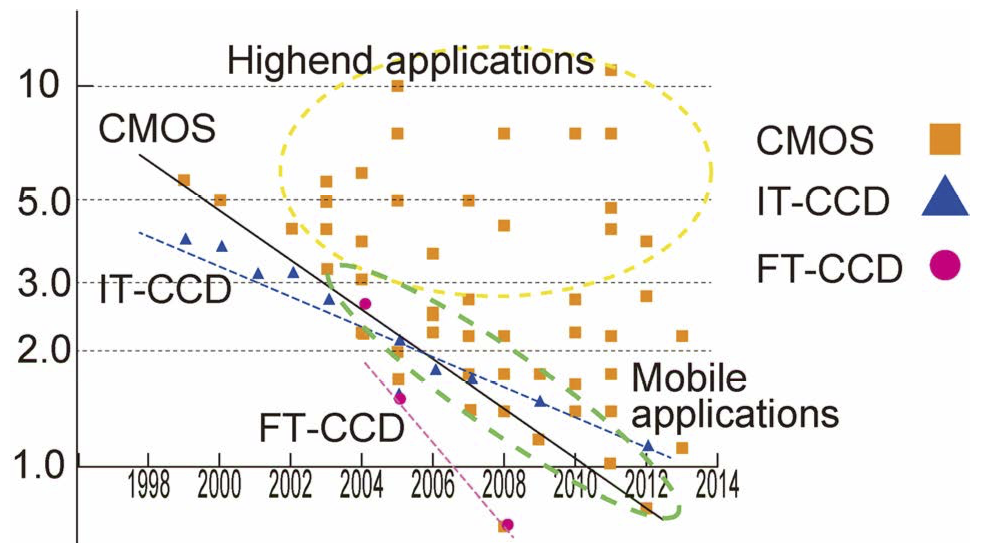
\includegraphics[width=0.45\textwidth]{figures/pixel_trend.png}
\caption[]{Trends in commercial sensor pixel sizes from \cite{isscc2016}}
\label{fig:pix_trend}
\end{figure}

CCD-based sensors still hold some performance advantages over CMOS sensors but the capability gap has narrowed almost entirely and the manufacturing and read-out rate advantages offered by CMOS have led to wholesale adoption in the consumer / commercial world.

When developing new remote sensing systems, the capabilities of modern commercial detectors promise the potential of smaller, less expensive systems with similar or better imaging performance to traditional TDI CCD-based systems.  However to realize this promise, the imaging system designer must consider the unique capabilities and shortcomings of the technology.

\subsection{Non-Imaging Commercial Electronic Trends}

In addition to the rapid advances in commercial imaging technology, Moore's law has continued to drive massive increase in microelectronic integration density with the associated performance, cost and device size improvements.

Indeed in recent years much of the emphasis has been in large-scale functional integration into single die "system-on-chip" (SoC) devices that operate at very high performance/watt for the consumer devices industry.  Such devices are uniquely enabling for small spacecraft in that, just as with consumer devices, they enable massive functionality in a small, low power package limit the amount of functional engineering "glue" required shortening design cycles.  Stated more directly, the computational power most people have in their pockets today was unavailable in large, complex spacecraft 10 years ago.

Similar arguments can be made for:

\begin{itemize}
    \item High density solid-state storage (Flash memory)
    \item Dedicated signal- and image-processing hardware for compression or computational imaging
    \item Digital modulation and radio technologies
    \item Inertial sensors
\end{itemize}

Indeed one can look at many of our personal consumer electronic devices and see the applicability to spacecraft in virtually every technology.  And these technologies have investment rates orders-of-magnitude higher than dedicated aerospace technologies.

Historically there has been resistance to the utilization of commercial electronics technologies for space applications due to reliability concerns, both intrinsic and due to the space environment.  Again, several things make such resistance less defensible:

\begin{itemize}
    \item High demonstrated statistical reliability of commercially-available components qualified to operate over thermal ranges much more severe than typical in-space environments (e.g. auto, industrial)
    \item Substantial improvement in CMOS latch-up susceptibility
    \item Deep and pervasive integration of hardware single-event protection driven by sea-level single-event susceptibility to massive integration devices
    \item Demonstration of high uptime and reliable operation of COTS-based avionics in LEO \cite{careful_cost}.
\end{itemize}

For small systems these trends are uniquely empowering and are more easily adoptable with lower cost (and hence less rsk-adverse) systems.

\section{Remote Sensing Metrics}
\label{sec:Metrics}
In order to compare different remote sensing systems, we need quantitative metrics.  The metrics we will introduce are fundamentally related to the data produced by such systems and are in two categories - \emph{quality} and \emph{volume}.  In a value-based assessment, quality and volume would form the numerator of a global value metric with cost in the denominator.

\subsection{Entendue and Photon Efficiency}
\label{sec:entendue}

Optical Entendue or throughput, $A \Omega$, is a fundamental space-bandwidth capacity metric for optics.  It is important because it captures the optical photon collection capacity of the optics. 

\begin{equation}
    P_{opt} = A\Omega \int_{\lambda_1}^{\lambda_2}L(\lambda) d\lambda = A\Omega L
\end{equation}

$A\Omega$ is also highly correlated with complexity and cost.  So a reasonable design objective is, given some optical entendue, extract the most imaging performance from the optics as possible.
Photons can be lost spatially if the detector area does not cover the full field of view (at the focal plane) of the optic or if there is non-unity duty cycle in photon integration.  Thus the effective usable photon power for imaging is:

\begin{equation}
    P_{img} = \eta_{ph} A \Omega L 
\end{equation}

where

\begin{equation}
    \eta_{ph} = \frac{A_{det}}{A_{fov}} \phi_{int}
\end{equation}

where $A_{det}$ is detector area, $A_{fov}$ is the area of the optical field of view at the focal plane and $\phi_{int}$ is the fraction of time that the detectors are actively integrating photons.  

$\eta_{ph} A \Omega$ is a fundamental imaging system capacity metric.  Various system trades can be made between image quality and area collection rate but these trades are all constrained within the boundaries of this fundamental system capacity.


\subsection{Image Quality}
\label{sec:iq}

Image quality is a complex, multi-faceted subject and while there is no perfect model or metric, substantial work has gone into quantifying the image quality of high resolution remote sensing systems.  Before jumping into integrated image quality models, we will define the geometric and radiometric components of image quality.

\subsubsection{Resolution, NIIRS and GIQE}
Resolution is a key component of image quality but is a surprisingly difficult-to-define metric.  Often Ground Sample Distance ($GSD$) is used as a proxy for resolution under the assumption that all pixels are created equally.  This assumption doesn't hold for systems with widely varying $SNR$ or sharpness (see Section \ref{sec:q}).

More holistic definitions of resolution typically refer back to \emph{resolvability} or the ability to distinguish objects or features of a given size in an image.  The so-called Ground Resolution Distance ($GRD$) is an example of a such a metric.  Unfortunately the definition of $GRD$ is not universally agreed to or consistent.  We will define a $GRD$ metric based on the NIIRS scale.

High resolution systems are typically evaluated by quantitative "image interpretability" scales the best known being the National Image Interpretability Rating Scale, or NIIRS.

NIIRS rating is described by specific human interpretation standards, examples of which are shown in Table \ref{table:NIIRS}\cite{niirs}.

\begin{table}[h!t]
\resizebox{.45\textwidth}{!}{%
\begin{tabular}{@{}lll@{}}
\toprule
\textbf{NIIRS} & \textbf{GRD}          & \textbf{Description}                                                                                                                             \\ \toprule
3     & 2.5m - 4.5m  & \begin{tabular}[c]{@{}l@{}}Identify a road as divided or undivided\\ Detect rows of automobiles in a parking lot\end{tabular}           \\ \midrule
4     & 1.2m - 2.5m  & \begin{tabular}[c]{@{}l@{}}Detect barriers/obstacles (barrels) on runways\\ Distinguish between locomotives and railcars\end{tabular}   \\ \midrule
5     & 0.75m - 1.2m & \begin{tabular}[c]{@{}l@{}}Identify individual lines painted on paved roads,  parking lots\\ Identify fallen utility poles\end{tabular} \\ \midrule
6     & 0.4m - 0.75m & \begin{tabular}[c]{@{}l@{}}Detect individuals, when not in a group\\ Detect small road signs in an urban area\end{tabular}              \\ \bottomrule
\end{tabular}%
}
\centering
\caption{NIIRS definitions}
\label{table:NIIRS}
\end{table}

NIIRS is a logarithmic scale traditionally evaluated by trained human image interpreters.  However, much work has gone into developing semi-analytic regressions to predict NIIRS from basic image quality parameters such as sharpness, signal-to-noise ratio (SNR), etc. The Generalized Image Quality Equation (GIQE) is an example of such a function; we will use the 5th version, GIQE-5 which is defined in eq. \ref{eq:giqe5}.

\begin{dmath}
NIIRS = 4.4 - 3.32 \log(GSD_{m}) + 3.32 \left[1 - e^{\frac{-5.308}{\Delta SNR}}\right]\log(RER_0)
- 0.402 \log(RER_0)^4 - 2.92/\Delta SNR - 0.069N_{smear}
\label{eq:giqe5}
\end{dmath}
where $GSD_{m}$\footnote{GSD units must be paid close attention to - many references list GIQE using units of inches for GSD.  In this case, the first parameter in the equation is 9.7 rather than 4.4 because $4.4 - 3.32\log{\left(39.4 \frac{in}{m}\right)} \approx 9.7$} is the ground sample distance in meters, $\Delta SNR$ is difference between $SNR$ for a 15\% and 8\% target reflectance, $RER_0$ is the raw Relative Edge Response (without sharpening or MTFC) and $N_{smear}$ is the number of pixels of linear smear.

GIQE-5 is fairly well validated again human interpreters \cite{giqe5} and nicely captures the trade-off between various imaging system parameters such as $SNR$ and $GSD$.  Note that GIQE-5 is logarithmic in resolution such that a halving of $GSD$ (proportional to resolution when holding other parameters constant) results in a NIIRS improvement of 1.

Based on this definition, one can use GIQE-5 to define $GRD$:

\begin{equation}
    GRD(m) = 10^{4.4 - \frac{NIIRS}{3.32}}
\end{equation}

\cite{auelmann_iq} shows that:

\begin{equation}
    GRD = \frac{R\times IFOV}{RER} = \frac{R\lambda_{mean}}{D_{ap} Q \times RER (Q)}
\label{eq:alpha_eff}
\end{equation}

and that a good approximation for the GIQE-based $GRD$ for diffraction limited systems is given by:

\begin{equation}
    GRD \approx \frac{R\lambda_{mean}}{D_{ap}}\left[1 + \frac{1}{Q^{1.35}}\right]^{1/1.35}
\label{eq:alpha_eff_approx}
\end{equation}

\includefigure{figures/resolution_q.pgf}{fig:resolution_q}{Relationship of GRD and GSD as resolution metrics as a function of Q}

Notice in Figure \ref{fig:resolution_q} that GRD asymptotes at $Q=2$ due to diffraction but that GSD continues decreasing monotonically.  This is because optical systems do not pass spatial frequency beyond the diffraction limit which is critically sampled at $Q=2$ and illustrates why GSD is a problematic resolution metric.

\subsubsection{Dynamic Range ($DR$) and Signal-to-noise Ratio ($SNR$)}
Dynamic range and signal-to-noise ratio are closely related by subtly different measures of radiometric performance.

Dynamic range is defined as the ratio of maximum-to-minimum signal level that the system can capture or represent in an image:

$$DR = \frac{S_{max}}{S_{min}}$$

The minimum signal level is the noise-floor of the system, $s_{min} = \sigma$ where $\sigma$ represents all non-signal-correlated noise sources in the system including read noise, dark current, etc.

The maximum signal is the maximum number of photo-electrons the system can capture for one output image pixel and is limited by the well depth of a pixel, $s_{max} = N_{e^-}^{well}$ for single-exposure systems.  Note that in digitally oversampled systems (covered later), the digital oversampling factor directlye expands dynamic range by increasing the effective well depth such that $s_{max} = N_s N_{e^-}^{well}$ where $N_s$ is the oversampling ratio.  Oversampling also affects $s_{min}$ and it can be shown that, for equally exposed samples:

\begin{equation}
    DR = \sqrt{N_s}\frac{N_{e^-}^{well}}{\sigma_{uncor}}
\label{eq:DR_OS}
\end{equation}

Dynamic range is a very important quality parameter for remote sensing systems because the dynamic range of terrestrial natural scenes can be quite high.  

\begin{figure}[h!]
\centering
\begin{subfigure}{0.31\linewidth}
\centering
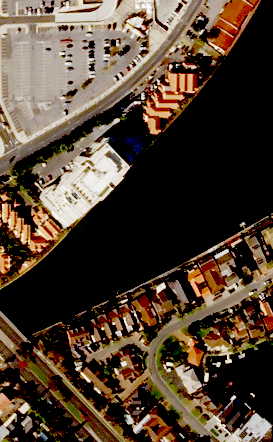
\includegraphics[width = \textwidth]{figures/pb_bad_dr_low.png}
\end{subfigure}
\begin{subfigure}{0.31\linewidth}
\centering
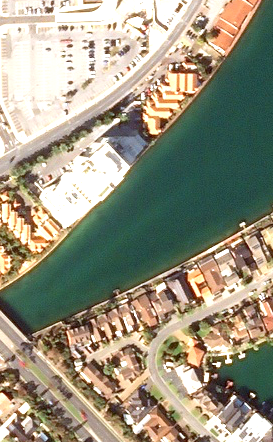
\includegraphics[width = \textwidth]{figures/pb_bad_dr_high.png}
\end{subfigure}
\begin{subfigure}{0.31\linewidth}
\centering
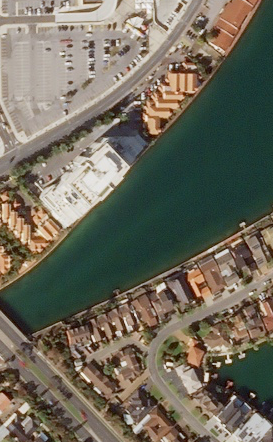
\includegraphics[width = \textwidth]{figures/pb_good_dr.png}
\end{subfigure}
\caption{The first two images have relatively low dynamic range.  The first is under-exposed and the second over-.  Note the details lost in shadows in the first and highlights (parking lot) in the second when compared with the third image which has about 100dB of DR}
\end{figure}

For systems that digitally oversample with unequal exposures, the dynamic range can be even larger as is shown in section \ref{sec:hdr}.

Signal-to-noise ratio, $SNR$, like dynamic range depends critically on both the detector well depth and its noise characteristics.  However signal-to-noise ratio is not purely a system-defined metric but depends also on the scene being imaged and as well as exposure parameters.  In general $SNR$ is defined as:

$$SNR = \frac{s}{\sigma_{noise}}$$

In general noise consists of the same sources discussed for $DR$ but also the shot-noise associated with the signal, $s$.  Because arrival rate of incoming photons obey Poisson statistics, it can be shown that $\sigma_{shot} = \sqrt{s}$ such that:

$$SNR = \frac{s}{\sqrt{\sum{\sigma_i^2} + s}}$$

In order to state an $SNR$, the signal, $s$, must be constrained by other system parameters and some exposure.  Typically $SNR$ is specified with respect to a specific target reflectance or top-of-atmosphere (TOA) radiance and a maximum or saturation reflectance or TOA radiance.  For a perfectly exposed scene with

$$\alpha = \frac{L_{typ}^\lambda}{L_{sat}^\lambda}$$
,
$$SNR_{\alpha} = \frac{\alpha N_{e^-}^{well}}{\sqrt{\sum{\sigma_i^2} + \alpha N_{e^-}^{well}}}$$

where $\alpha$ is the ratio of target radiance (or reflectance) to the saturation value.  This relation, like $DR$, can be expanded to include multiple digital exposures such that

\begin{equation}
\label{eq:snr_alpha_multiframe}
SNR_{\alpha} = \sqrt{N_s}\frac{\alpha N_{e^-}^{well}}{\sqrt{\sum{\sigma_i^2} + \alpha N_{e^-}^{well}}}
\end{equation}

For most modern detectors, uncorrelated noise sources are small compared with shot noise so we can approximate eq. \ref{eq:snr_alpha_multiframe}

\begin{equation}
\label{eq:snr_alpha_multiframe_simp}
SNR_{\alpha} \approx \sqrt{N_s \alpha N_{e^-}^{well}}
\end{equation}

\subsection{Collection Capacity}
\label{sec:capacity}
For a spacecraft, system collection capacity is constrained by a delicate balance between image collection capacity and the ability to get the collected data to the ground.  The latter is dictated entirely by data intensity, $I_D$, and communications bandwidth (which we won't go into here).  

Image collection capacity in turn depends on a number of parameters including time over land, ACS agility, and area collection rate,

$$ACR = V_{gnd}W_{ct}$$

where $W_{ct}$ is the swath width or cross-track field of view projected to the ground

We will define a collection duty cycle metric that captures all of the impacts on collection capacity outside of the system $ACR$ as:

\begin{equation}
    \beta = \frac{t_{collect}}{t_{per}}
\end{equation} 

where $t_{per}$ is the spacecraft orbital period and $t_{collect}$ is the collection time per orbit.  Note that $\beta$ is itself dependent on $V_{gnd}$ in addition to a wide variety of targeting-related parameters such as time per orbit over land and in the sun, average target cross-track spacing (for targetted spacecraft), attitude control bandwidth, etc.

For targeting remote sensing systems constrained by sun and time-over-land, typically $\beta < 0.1$ as shown in Fig. \ref{fig:beta}

\includefigure{figures/collection_dc.pgf}{fig:beta}{Collection Duty Cycle, $\beta$, for various cross-track target spacings for a reasonably agile spacecraft}

We can similarly define a downlink duty cycle

\begin{equation}
    \gamma = \frac{t_{d/l}}{t_{per}}
\end{equation}

where $\gamma$ is typically $\sim 0.1$ for a single ground station well matched in latitude to the spacecraft's orbit inclination and can be increased with additional, geographically diverse ground stations.

There are two primary capacity regimes that a spacecraft may operate in:

\begin{enumerate}
\item Downlink-constrained regime
\item Collection-constrained regime
\end{enumerate}

We can define a capacity constraint metric, $k_{cap}$

\begin{equation}
k_{cap} = \frac{\gamma BW_{d/l} GSD^2}{\beta I_D ACR}
\end{equation}

such that when $k_{cap} < 1$ the system is \emph{downlink constrained} and when $k_{cap} \geq 1$, the system is \emph{collection constrained}.

For a commercial system with multiple ground stations and a dense target deck, a reasonable rule-of-thumb is that $\frac{\gamma}{\beta} \approx 3$ so that a well balanced system has:

\begin{equation}
    BW_{d/l} \approx \frac{I_D ACR}{3 GSD^2}
\end{equation}

\subsection{Data Intensity}

Data intensity, $I_D$, is a metric that impacts a wide range of spacecraft subsystems from on-board storage and data handling to downlink bandwidth.  It is defined as the number of digital bits captured, processed or transmitted per image product output pixel

$$I_D \equiv \frac{N_{bit}}{N_{px}^{L1b}}$$

Where we assume an output product to consist of the fused, corrected but un-rectified L1b product. For a typical imaging pipeline that includes compression we must define exactly where in the system $N_{bit}$ is defined.  We will use the post-compression image data because it impacts the most system interfaces (storage, downlink, processing) and is generally directly proportional to the raw pixel data rate through the compression ratio, $C$

\begin{equation}
    \label{eq:compression}
    C \equiv \frac{N_{bpp}^{raw}}{N_{bpp}^{comp.}}
\end{equation}

For a digitally oversampling system

\begin{equation}
    I_D = N_s N_{bpp}^{comp.} = \frac{N_s N_{bpp}^{raw}}{C}
\end{equation}

Note also that any resampling operations (including image reconstruction techniques such as super-resolution) impact $I_D$ because for non-unity resampling ratios the number of output pixels is affected.  Thus we include a resampling factor

$${\eta}_{rs} = \frac{GSD_{L1b}^2}{GSD_{L0}^2}$$

such that

\begin{equation}
    \label{eq:I_D}
    I_D = {\eta}_{rs} N_s N_{bpp}^{comp.}
\end{equation}

We can also define a collect-area normalized data intensity, $I_A = \frac{I_{D}}{GSD^2}$.  Given eq. \ref{eq:I_D}

\begin{equation}
    I_A = \frac{N_s N_{bpp}^{comp.}}{GSD_{L0}^2}
\end{equation}

Finally, it is worth noting that for a system with well-matched analog and digital (quantization) dynamic range

\begin{equation}
    N_{bpp}^{raw} \sim \textrm{log}_2(DR^{raw})
\end{equation}

\section{Performance Trade Space}
\label{sec:trade_space}

The remote-sensing trade space is largely constrained by four mission needs:

\begin{enumerate}
\item Phenomenology
\item Image Quality
\item Collection Capacity
\item Cost
\end{enumerate}

\emph{Phenomenology} refers to the study of the phenomenon being sensed and goes beyond Image Quality to include things like the spectral content of the sensed data.  We will largely discuss the trade space in terms of wide-bandwidth ($>100nm$) collection in the near-visible spectrum ($\sim 400nm$ to $\sim 1000nm$) but will also point out where the trends in questions impact the ability to perform other phenomenology (e.g. SWIR or HSI).

\emph{Image Quality (IQ)} and \emph{Collection Capacity} are tightly coupled at the system level.  We will discuss each and their relation to each other in more detail later, but to motivate the tradeoffs, we note the following result derived in \cite{shaw}

\begin{equation}
    \label{eq:acr_scaling}
    ACR \propto \frac{GSD^4}{SNR^2 \times N_{\lambda}^2}
\end{equation}

where is $ACR$ is Area-Collection-Rate in land area per time, $N_{\lambda}$ is the number of spectral bands the full spectral bandwidth is divided into.  

Equation \ref{eq:acr_scaling} very effectively demonstrates the deep relationship of image quality ($GSD$ and $SNR$) and collection capacity for a set of other system parameters.  It also forms the basis for a useful overall system performance and complexity figure-of-merit:

\begin{equation}
    \label{eq:perf_complex_metric}
    FOM = \frac{ACR \times SNR^2 \times N_{\lambda}^2}{GSD^4}
\end{equation}

\subsection{Pixel Size and Q}

The first technology observation we made regarded pixel size or pitch, $p_{px}$ and its impact on image quality, collection capacity and system characteristic size and, hence, cost.  We will study the effect of pixel size through the lens of $Q$ recognizing that

$$Q \propto \frac{f}{p_{px}}$$

and then show why driving Q with pixel size is preferable to focal length, $f$ or diameter, D.

$Q$ is generally chosen as a trade between image quality, collection capacity and system size.  

In \ref{sec:iq} we show that the NIIRS as predicted by the Generalized Image Quality Equation (GIQE-5) is a useful image quality metric for remote sensing systems.

\includefigure{figures/Q_iq.pgf}{fig:q_iq}{Parametric study of GIQE-5 shows how optimal image quality depends on Q.  Note that this plot assumes $RER_0 = 0.3$ and $GSD = 1m$ for $Q=1$ and that $SNR \approx 1 / Q$}

One thing demonstrated in parametric study of the GIQE-5 is that image quality is often maximized at $Q>1$ (Fig. \ref{fig:q_iq}).  This has also been validated in human-interpreter studies \cite{fiete_Q_IQ} and is not unexpected considering that in a diffraction-limited system with $Q<2$, there is contrast passed by the optical system that is not sampled by the detector.  At first blush it seems obvious that, given the cost and difficulty of building larger optics, systems would be designed at $Q>1$.  However, there are three other system impacts of $Q$ that make pushing $Q$ higher problematic.

The first is that for CCD-based TDI systems, pixels with sufficient full well capacity ($FWC$), and hence $SNR$ performance have required $p_{px} >> 10um$.

The second is that given other system constraints (detector line rate, $SNR$ required, focal plane dimension) [TODO: verify this relationship is right!!]

\begin{equation}
    ACR \propto \frac{1}{Q^2}
\end{equation}

Finally, other constraints being equal

\begin{equation}
    SNR \propto \frac{1}{Q}
\end{equation}

if pixel pitch of FWC is considered (see section \ref{sec:FWC_px}) is considered.

Thus designers have tended to accept lower $Q$, and hence larger $GSD$ and poorer image quality in exchange for manageable optical focal lengths, increased area collection capacity and acceptable $SNR$ / $DR$.

\begin{observation}[$Q > 1$]
Image Quality is optimized for $Q>1$ but because $ACR \sim 1/Q^2$ and systems were pixel-size limited, historical systems typically been developed at $Q<1$.
\end{observation}

Happily, the trend towards much smaller pixel in commercial image detectors (Fig. \ref{fig:pix_trend}) opens up the opportunity of driving to towards higher $Q$'s where image quality is optimized without increasing system size.

Smaller pixels typically store less charge, both in the photodector and storage node. In fact to first order\cite{jerram}:

\begin{equation}
  \label{eq:pix_fwc_scaling}  
N_{e^-}^{FWC} \propto p^2
\end{equation}

\includefigure{figures/p_fwc.pgf}{fig:p_fwc}{Relationship of $N_{e^-}^{FWC}$ to pixel size, $p_{px}$.  Note that while scaling generally follows eq. \ref{eq:pix_fwc_scaling}, there are notable outliers especially in some of the new CMOS architectures}

and while there are process optimizations that can improve this, these typically are second order to simple area scaling.  Fig \ref{fig:p_fwc} shows that this trend is reasonably well supported although several recent pixel architectures are significant outliers.

This leaves the challenge of achieving acceptable $SNR$ and $DR$ and we will show in section \ref{sec:modalities} that the high data sampling rates of modern CMOS pixels coupled with analog stabilization enables this at high $Q$ and with small pixels.

And so we also argue that:
\begin{observation}[Trend Towards Smaller Pixels and Hybrid Stabilization]
\label{obs:small_pix}
Smaller pixels enable driving system size down and $Q$ up but require hybrid stabilization (digital + analog) to make practical due to inherently lower signal, $S$ obtained during exposure.
\end{observation}

\section{Collection Modalities}
\label{sec:modalities}
Large orbital velocity is a large advantage of spacecraft for remote sensing over other platforms as it gives:


\begin{itemize}
\item Daily global access
\item High collection rates
\end{itemize}

However it also presents large challenges in developing an imaging system that can collect sufficient light at the high relative scene velocity without incurring unreasonable blur.

For blur-limited integration times, in can be shown that \cite{shaw}

$$SNR \propto \frac{D_{ap} GSD^{3/2}}{\sqrt{V_{gnd}}}$$

Or if $SNR$ is a fixed requirement, relative ground velocity must be reduced such that:

\begin{equation}
V_{gnd} \propto GSD^3
\end{equation}

which has many system-level impacts, the largest of which is its impact on area collection rate, $ACR$:

$$ACR \propto V_{gnd}$$

This is a major challenge for high-resolution systems and historically there have been many solutions to compensate for scene motion on spacecraft.  These date back to the earliest film-based systems that used the film motion through the camera itself to compensate.  Other mechanical solutions included gimbaled cameras, "back-scan" of the entire spacecraft bus and full-aperture scan mirrors among others.

Indeed for systems with resolutions better than a few meters, some form of stabilization is essentially required to obtain sufficient $SNR$ without significant bus back-scan to reduce relative ground velocity.

We will classify modern stabilization strategies into three major buckets

\begin{enumerate}
\item Analog electronic charge transfer or time-delayed integration (TDI) stabilization
\item Digital oversampling stabilization
\item Analog optomechanical stabilization
\end{enumerate}

Digital imaging spacecraft have traditionally used a "push-broom" architecture where a line-array sensor is pushed along the ground by the spacecraft's motion.  Stabilization by charge transfer between rows synchronous with scene velocity allows for so-called Time Delayed Integration TDI.  

Development of large format CCD and CMOS framing detectors allow for  "step-and-stare" architectures in which a scene snapshot is captured with a 2D framing sensor that is then moved further along the orbital path before another scene is captured.  If the framing rate is high enough, the scene can be digitally oversampled such that a single point on the ground is captured with multiple exposures of the focal plane.

\begin{figure}[h!t]
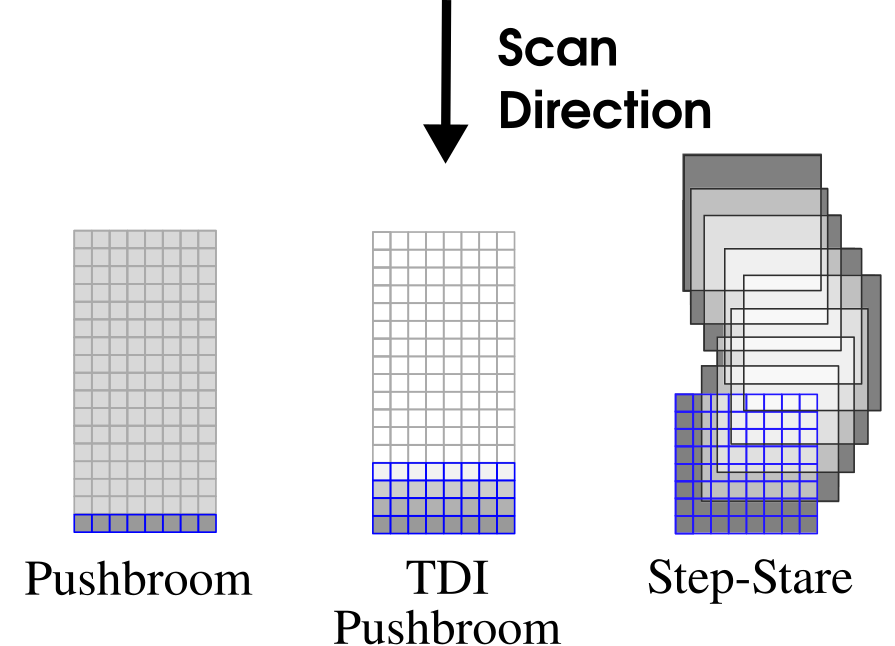
\includegraphics[width=0.42\textwidth]{figures/modalities.png}
\caption{General satellite imaging modalities}
\label{fig:modalities}
\end{figure}

Analog optomechanical stabilization relies on an optomechanical component with the ability to dynamically steer the payload line of sight repetetively so as to remove relative scene motion during integration.  Fast scan mirrors (FSM) or excited dynamic motion of the entire instrument are two ways to achieve this \cite{patent:jonny}, \cite{patent:dirk}.

The analog techniques are considered such because they occur before digital sampling of the detectors and are thus still limited by detector well capacity.  Digital oversampling is not as constrained by $FWC$ beause each exposure resets the pixel and thus is the $FWC$ can be effectively expanded by as many redundant samples as can be obtained.

Both TDI pushbroom and step-and-stare allow for some form of stabilization or motion compensation which is required to obtain reasonable $SNR$ in high resolution systems.  In the case of Figure \ref{fig:modalities}, analog charge transfer is depicted for TDI pushbroom and digital oversampling (through overlapping frames) is depicted for step-and-stare.  Pushbroom is shown mostly for historical reference as pure pushbroom collection is not feasible in systems with $GSD$ much below 10m.

To-date analog electronic or TDI stabilization has only been implemented successfully in CCD detectors.  There is ongoing work to implement TDI in CMOS detectors but this technology is still immature - see \ref{sensor_tech}.  

Likewise digital oversampling is typically not practical using CCD sensors in high resolution systems due to the inherent limitations on read-out rate of CCD as compared with CMOS technology.

Finally it is important to point out that digital and analog stabilization can be combined in the same system.  Such hybrid stabilization schemes could be in the form of analog opto-mechanical stabilization plus digital oversampling or a TDI CCD that is read out fast enough to allow digital oversampling.  Indeed we will argue later that such hybrid stabilization schemes uniquely leverage the capabilities of modern CMOS detectors, enable smaller systems and provide significant system-level flexibility.

\subsection{Analog Stabilization with TDI}

TDI systems are based on a unique property of CCD image sensors - their ability to move charge between nodes at very high charge transfer efficiency (CTI) and without incurring significant noise in the process.  In fact TDI sensors essentially enabled the move away from film in the classified systems of the 1970's.

Typical TDI sensors will have anywhere from 4 to 256 "stages" each consisting of a row of pixels covering the swath width.  The rows are oriented normal to the scan direction and charge is shifted row-to-row synchronously with the scene motion such that the effective integration time for a point on the ground is multiplied by the number of stages in the device.  Figure \ref{fig:tdi} illustrates this mode for an 12-stage TDI detector in t-x space where x is in-track dimension.

\includefigure{figures/tdi.pgf}{fig:tdi}{TDI t-x diagram.  Red row indicates one in-track ground sample}

In general TDI system's photon collection efficacy is "well-depth limited" meaning that the duration of integration is typically limited by pixel well saturation before other factors such as number of TDI stages, dark current, charge transfer efficiency.  For an appropriately exposed scene, the well-limited signal level is quite simple:

\begin{equation}
s = \alpha N_{e^-}^{FWC}
\label{eq:well_limited}
\end{equation}

Noting that the exposure time for a single stage of a TDI system is extrinsically related to the linerate, $LR$ $t_{int}^{line} = \frac{1}{LR}$, and noting that $t_{int} = N_{TDI}t_{int}^{line}$, we can combine with equation \ref{eq:s} to obtain an expression for optimal number of TDI stages:

\begin{equation}
N_{TDI} =\frac{N_{e^-}^{FWC} Q^2}{k_{pe} L_{sat}}\frac{LR}{QE} \propto \frac{N_{e^-}^{FWC}V_{gnd}}{D_{ap}^2 GSD^3 L_{sat}}
\label{eq:n_tdi}
\end{equation}

Figure \ref{fig:n_tdi} below shows this trade.

\includefigure{figures/N_tdi.pgf}{fig:n_tdi}{Optimal TDI stages vs. resolution and Q}

While extremely powerful and well-proven over many missions, TDI detectors present challenges for low-cost, high resolution missions.

Historically missions have developed custom TDI detectors due to the unique performance and mission requirements of a spacecraft\cite{jerram}.  These include high line rates, large full-well capacity, low read-noise, high quantum-efficiency and radiation tolerance.  And while there are commercially available TDI detectors, they typically do not meet the requirements of high resolution collection from a space platform.

As we noted in Observation \ref{obs:small_pix}, smaller pixels are desirable from a system-size perspective but this typically comes at the expense of pixel full-well capacity, especially in off-the-shelf CCD's.  We show in section \ref{sec:eta_ph} that this limitation can be overcome through digital oversampling. 

However, because TDI systems inherently couple stabilization rate, integration time and read-out line rate, digital oversampling is not an option with a single TDI array, limiting dynamic range.  The limited dynamic range is also compounded by inflexibility in exposure which is entirely constrained by the line rate and number of TDI stages.  

\subsection{Digital Stabilization with Step-and-Stare}
Step and stare relies on a high speed framing CMOS sensor to capture multiple, overlapping frames of the same point on the ground as the scene moves by.  The redundant samples are then re-combined in post-processing to creat output data with a longer effective integration time - virtual TDI in a way.

\includefigure{figures/step_stare.pgf}{fig:step_stare}{Step-and-stare t-x diagram.  Red row indicates one in-track ground sample}

Figure \ref{fig:step_stare} illustrates this mode on a t-x diagram.  Note that for visualization we illustrate a detector height of only 36 pixels in and a very high framing rate whereas in reality most modern framing sensors are > 1000 pixels high and frames at about 1/6 of the rate shown.  Fig. \ref{fig:step_stare_real} shows the same thing with realistic frame height and framerate illustrating the extremely low imaging duty cycle.

It is worth noting in this diagram that the photon collection duty cycle, $\phi_{ph}$ is small, especially compared with a traditional TDI system which is essentially 100\%.  This can be seen in the white gaps between integrations.  It is also worth noting the slanted integration periods indicative of motion blur during integration.  Single frame integration time (and thus SNR) for step-and-stare is typically limited blur-limited (see \ref{sec:eta_ph}).  This is a problematic limitation and severe enough that systems $GSD$ below about 3m must reduce $V_{gnd}$ with a bus "back-nod" in order to get sufficient signal without incurring substantial blur.

\includefigure{figures/step_stare_real.pgf}{fig:step_stare_real}{Step-and-stare t-x diagram with realistic array height and framerate.}

However step-and-stare IS NOT limited by small pixel FWC as each the well is read out in each independent integration and then summed digitally.  Thus the advantages and disadvantages of step-and-stare compared with TDI can be summarized as:


\subsection{Hybrid Step-and-stare / analog opto-mechanical stabilization}

\includefigure{figures/stab_step_stare.pgf}{fig:stab_step_stare}{Stabilized Step-and-Stare t-x diagram.  Red row indicates one in-track ground sample}

\subsection{$\eta_{ph}$ and Comparison of modalities}
\label{sec:eta_ph}

One way to conceptualize $\eta_{ph}$ for the different modalities is as the time-average (or integral over time) of the blue areas in Figures \ref{fig:tdi}, \ref{fig:step_stare}, \ref{fig:step_stare_real} and \ref{fig:stab_step_stare}.  Increasing in-track height of the blue bars with taller arrays helps improve this integral and reducing the gaps between them horizontally (in time) improves this.  TDI has a time-duty cycle of 1. (no horizontal gaps) while step-and-stare typically have much taller arrays.

In order to quantify this it can be shown that

$$A_{fov} = D_{ap}^2 \left(F^\# \right)^2 \Omega = f^2 \Omega $$

or 

$$A_{fov} = \pi D_{ap}^2 \left(F^\# \right)^2 \theta_{fov}^2 = \pi f^2 \theta_{fov}^2$$

where $\theta_{fov}$ is the conical field of view in the small angle approximation.

From this, we can derive $\eta_{ph}$ for systems in two regimes: blur constrained and full-well capacity constrained.  The domains are separated by the following criteria:

\begin{align*}
    N_{e^-}^{FWC} &>& \frac{k_{pe}L_{sat}QE N_{bl} GSD}{Q^2 V_{gnd}} & \rightarrow &  \textbf{Blur-constrained} \\
    N_{e^-}^{FWC} &\leq& \frac{k_{pe}L_{sat}QE N_{bl} GSD}{Q^2 V_{gnd}} & \rightarrow &  \textbf{FWC-constrained}
\end{align*}

\includefigure{figures/blur_fwc_regime.pgf}{fig:eta_regime}{Representative regime map as a function of $GSD$ and $V_{gnd}$}

Figure \ref{fig:eta_regime} is a regime map for a set of reasonable parameters.

For the full-well capacity-dominated regime

\begin{equation}
    \label{eq:eta_ph_fwc}
    \eta_{ph}^{FWC} = \frac{\lambda^2 h_{px} N_{e^-}^{FWC} LR}{\pi D_{ap}^2 \theta_{fov}^2 k_{pe}(L)(QE)}
\end{equation}

which we can simplify to observe

\begin{equation}
    \label{eq:eta_fwc_scaling}
    \eta_{ph}^{FWC} \propto \frac{1}{D_{ap}^2 \theta_{fov}^2} \frac{N_{e^-}^{FWC} LR}{(L)(QE)}
\end{equation}

For high resolution systems without analog stabilization (digital stabilization or pure step-and-stare), radiometry is typically constrained by in-track blur due to the high apparent motion in the focal plane rather than the limited FWC of the pixel (Fig. \ref{fig:eta_regime}).  In this case,

\begin{equation}
    \label{eq:eta_ph_blur}
    \eta_{ph}^{bl} = \frac{\lambda^2 h_{px}N_{bl}(LR)(GSD)}{\pi D_{ap}^2\theta_{fov}^2 Q^2 V_{gnd}}
\end{equation}

Or 

\begin{equation}
    \label{eq:eta_blur_scaling}
    \eta_{ph}^{bl} \propto \frac{1}{D_{ap}^2 \theta_{fov}^2} \frac{N_{blur} (LR) (GSD)}{Q^2 V_{gnd}}
\end{equation}

This scaling law is not good for high resolution systems, requiring high $\frac{LR}{V_{gnd}}$ (and commensurate large data intensity, $I_{D}$), $N_{bl} >> 1 \: \textrm{px}$ or very low $Q$.

\begin{observation}[Design for FWC-limited regime]
Operation in the FWC-limited regime results in higher $\eta_{ph}$ and thus should be a design goal.
\end{observation}
and thus
\begin{observation}[The need for analog stabilization]
Analog stabilization is likely required to fully realize the advantages provided by high read-out rate, small pixel staring detectors.
\end{observation}

\subsubsection{CMOS Detectors enable increased $\eta_{ph}$}

Per eq. \ref{eq:eta_ph_fwc}, we note that 

\begin{equation}
    \eta_{ph}^{FWC} \propto h_{px}N_{e^-}^{FWC}LR
\end{equation}

High efficiency FWC-limited systems must either have larger full-well capacities or higher line-rates.  We observed earlier (Observation \ref{obs:small_pix}) that smaller pixels have positive system-level size (and thus cost) impacts and thus one desires focal planes with small pixels and high effective line-rates (where effective line-rates for staring arrays is defined in eq. \ref{eq:lr_framing}).

In light of this we define a sensor figure of merit

\begin{equation}
    \psi_{px} = \frac{h_{px}N_{e^-}^{FWC}LR}{p_{px}}
\end{equation}

$\psi_{px}$ is computed for a number of commercial-off-the-shelf sensors and plotted in Fig. \ref{fig:psi_px}.

\includefigure{figures/p_kpi.pgf}{fig:psi_px}{Detector figure of merit, $\psi_{px}$.  Note log scale and general trend of higher $\psi_{px}$ for CMOS sensors.}

Modern CMOS sensors are t

\begin{observation}[CMOS detectors coupled with analog stabilization are enabling]
The trend towards small pixels and high read-out rates enables CMOS detectors to extract more information from high performance, compact (and thus low cost) optics.
\end{observation}

\subsubsection{Relationshp of $\eta_{ph}$ to $ACR$ and $IQ$}

It can be shown that the total photo-electron generation rate, $\dot{N}_{e^-} \propto L\eta_{ph}A_{ap}\Omega$ and for FWC-limited systems operating in the shot-limited noise regime

\begin{equation}
    \dot{N}_{e^-} = \frac{ACR \times SNR^2}{GSD^2}
\end{equation}

such so that we can say

\begin{equation}
    \frac{ACR \times SNR^2}{GSD^2} \propto \eta_{ph} A_{ap}\Omega L
\end{equation}

This relationship demonstrates that $\eta_{ph}A_{ap}\Omega$ is a fundamental performance constraint for a remote sensings system within which trades between collection area and image quality can be made.

\subsubsection{Relationship of $\eta_{ph}$ to $I_{D}$ and $I_A$}

It is interesting to note that the relationship of $\eta_{ph}$ to data intensity is regime dependent as well.  In the blur-limited regime, it can be shown that:

\begin{equation}
    I_D \propto 
\end{equation}

Table \ref{table:modalities} summarizes qualitatively the relative advantages and disadvantages of the three modalities with detailed analysis of each in the following sections.

\begin{table}[h!t]
\resizebox{.45\textwidth}{!}{%
\centering
\begin{tabular}{@{}rccccc@{}}
\multicolumn{1}{l}{}                                                 & \textbf{DR}                       & \textbf{SNR}                        & $\eta_{ph}$         & \textbf{\begin{tabular}[c]{@{}c@{}}Stability\\ Req'd\end{tabular}} & \textbf{\begin{tabular}[c]{@{}c@{}}Data\\ Intensity\end{tabular}} \\ \cmidrule(l){2-6} 
\textbf{\begin{tabular}[c]{@{}r@{}}Analog \\Electronic\end{tabular}}                                                         & {\color[HTML]{F56B00} \textbf{-}} & {\color[HTML]{32CB00} \textbf{+}}   & {\color[HTML]{FE0000} \textbf{-}} & {\color[HTML]{FE0000} \textbf{- -}}                                & {\color[HTML]{32CB00} \textbf{++}}                                \\ \midrule
\textbf{\begin{tabular}[c]{@{}r@{}}Digital\\Oversampling\end{tabular}}                                                  & {\color[HTML]{32CB00} \textbf{+}} & {\color[HTML]{FE0000} \textbf{- -}} & {\color[HTML]{FE0000} \textbf{-}} & {\color[HTML]{32CB00} \textbf{++}}                                 & {\color[HTML]{FE0000} \textbf{- -}}                               \\ \midrule
\textbf{Hybrid} & {\color[HTML]{32CB00} \textbf{+}} & {\color[HTML]{32CB00} \textbf{++}}  & {\color[HTML]{32CB00} \textbf{+}} & {\color[HTML]{32CB00} \textbf{Tunable}}                            & {\color[HTML]{32CB00} \textbf{Tunable}}                           \\ \bottomrule
\end{tabular}%
}
\caption{Relative advantages, disadvantages of the modalities. $DR$ is dynamic range, $SNR$ is signal-to-noise ratio}
\label{table:modalities}
\end{table}
\subsubsection{High Dynamic Range Imaging}
\label{sec:hdr}

\section{Conclusions}
\label{sec:conclusions}

\section{Appendix A: Definitions}
\label{sec:appendix_a}

\subsection{Remote Sensing Driving Requirements}
\label{sec:requirements}

Table \ref{table:drivers} shows the effect of many mission-level needs on lower-level requirements.
\begin{table}[h!t]
\resizebox{.45\textwidth}{!}{%
\begin{tabular}{@{}ll@{}}
\toprule
\textbf{Requirement} & \textbf{Drives} \\ \toprule
Resolution & \begin{tabular}[c]{@{}l@{}}Aperture Diameter\\ Altitude\\$Q$\end{tabular} \\ \midrule
\begin{tabular}[c]{@{}l@{}}SNR \& Dynamic Range\end{tabular} & \begin{tabular}[c]{@{}l@{}}Stabilization\\ Detector Full-well\\Optical $F^\#$\end{tabular} \\ \midrule
Swath Width & \begin{tabular}[c]{@{}l@{}}Optical Complexity\\ Detector Width\\ Data Volume\end{tabular} \\ \midrule
Collection Rate & \begin{tabular}[c]{@{}l@{}}Stabilization\\ Detector line-rate\end{tabular} \\ \midrule
Spectral Sampling & \begin{tabular}[c]{@{}l@{}}In-track FOV\\ Camera filters\\ Semiconductor Bandgap\end{tabular} \\ \bottomrule
\end{tabular}%
}
\centering
\caption{System Performance Drivers}
\label{table:drivers}
\end{table}

\subsection{$\frac{\lambda F^\#}{p}$ or Q}
\label{sec:q}

The system parameter $Q$ is defined as:

\begin{equation}
Q = \frac{\lambda F^\#}{p}
\label{eq:Q}
\end{equation}
and is essentially a measure pixel sampling in the spatial domain relative to the Nyquist criterion.  Nyquist says that to completely reconstruct a band-limited system, the spatial sampling frequency. 
$$\rho_s = 1/p \geq 2 BW_{opt}$$

Because we always sample to DC, the optical bandwidth $BW_{opt}$ is replaced by the diffraction cutoff frequency.
$$\rho_c = \frac{1}{\lambda F^\#}$$

Thus $Q$ is a measure of Nyquist sampling where $Q=2$ is critically sampled.  Most systems, however, operate at $Q < 2$ and hence incur some spatial aliasing.  There is little reason to operate at $Q > 2$ as the optics do not pass spatial frequency information there so the additional sampling is essentially wasted.

\begin{figure}[h!]
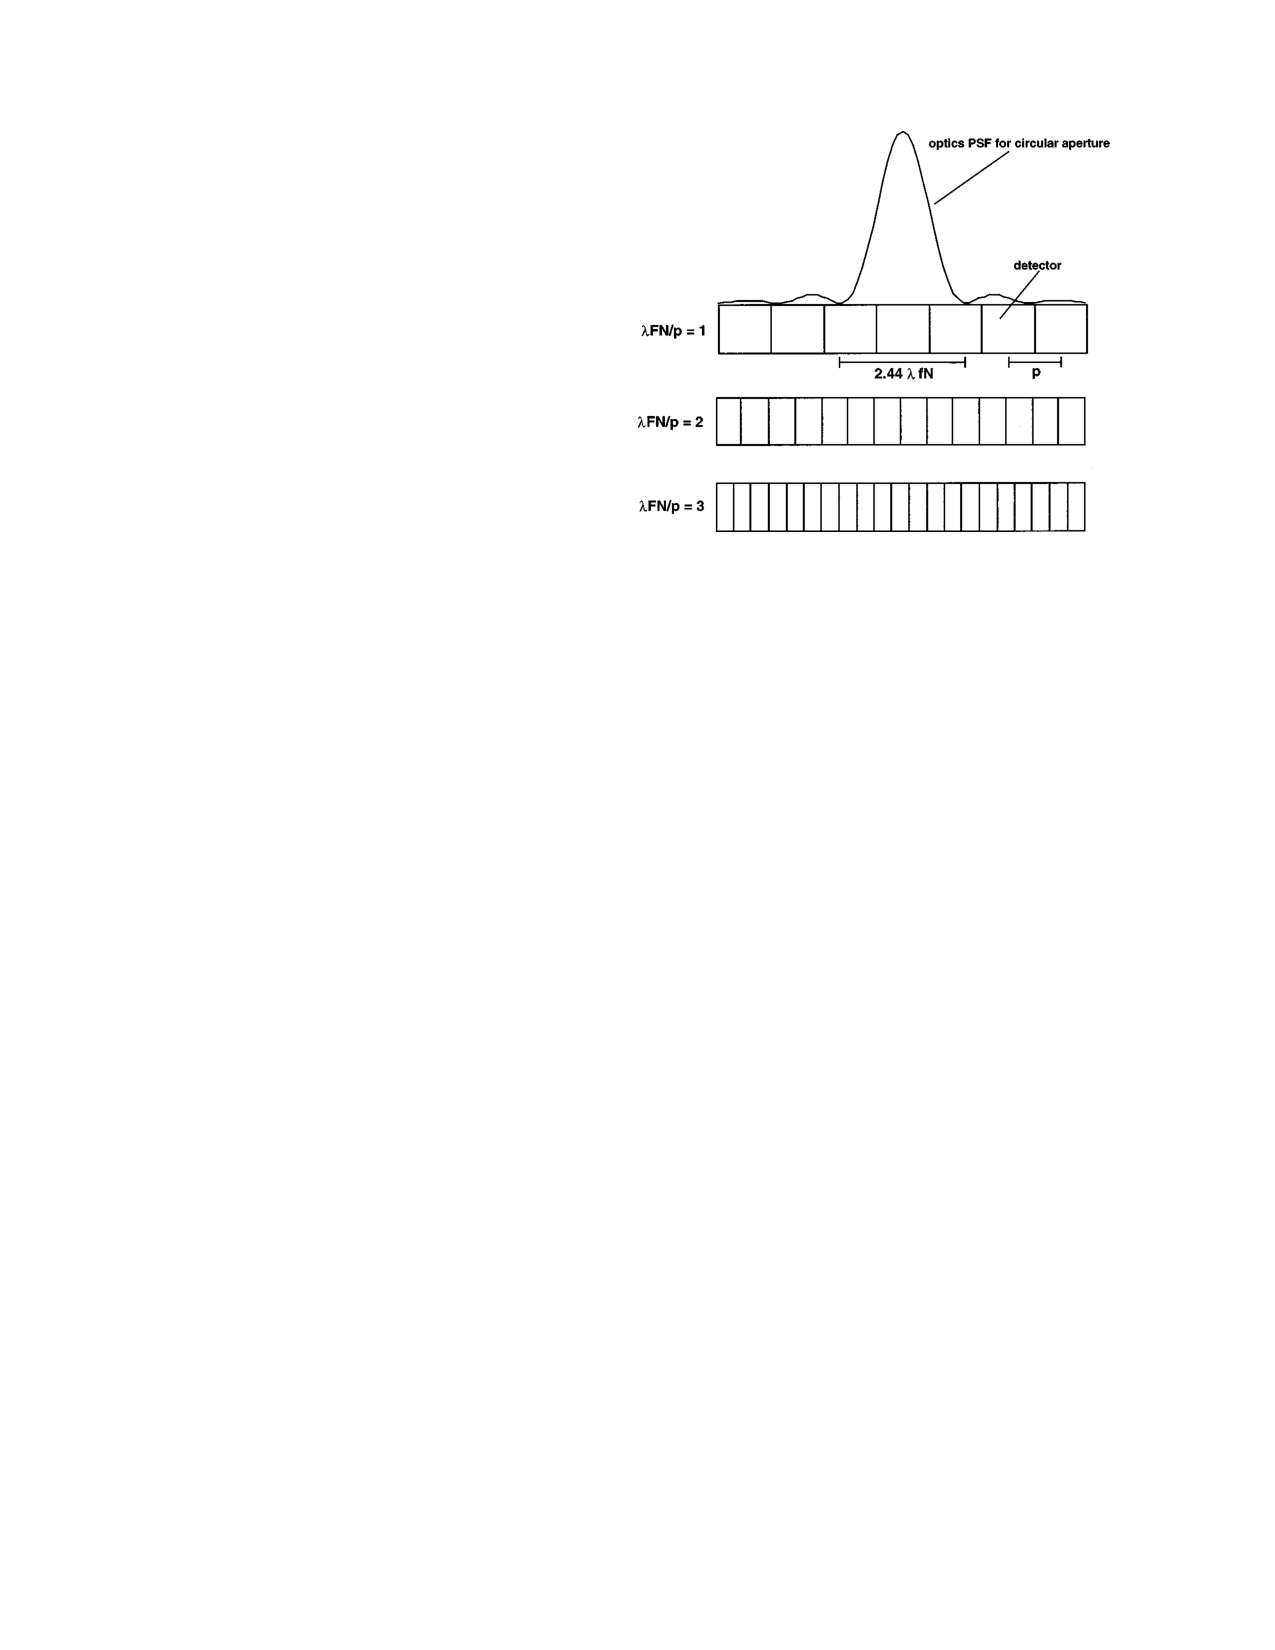
\includegraphics[width=0.42\textwidth]{figures/Q_fiete.pdf}
\caption{Spatial interpretation of Q sampling a diffraction-limited PSF.  Adapted from \cite{fiete_q})}
\end{figure} 

Beyond a statement of the Nyquist criterion, $Q$ is a very useful parameter by which to evaluate and compare systems.  For more see \cite{fiete_q}.  

\subsection{Photon Radiometry}

In order to not have to carry full radiometry for every calculation, we will define a payload photo-electron gain, 

\begin{equation}
k_{pe} \equiv \frac{\dot{N}_{e^-}^{std}}{L}
\label{eq:k_pe}
\end{equation}

Where 

\begin{equation*}
    L = \int_{\lambda_1}^{\lambda_2}L_{\lambda}(\lambda)d\lambda
\end{equation*}

is radiance at aperture in W/m$^2$-sr, $QE$ is quantum efficiency, $\Delta \lambda$ is spectral bandwidth and $\dot{N}_{e^-}^{std}$ is photo-electron generation rate for the case of $QE=1$, $Q=1$.

Moving forward, we will use $k_{pe} = 2\times 10^5$ e$^-$-sr-um-m$^2$/J\footnote{Given $\Delta \lambda = 0.5$um, $L = 100$ W/m$^2$-sr-um, this equates to $\dot{N}_{e^-}^{std} = 1\times 10^7$ e$^-$ / s or 5,000 photo-electrons accumulated in a 1ms integration time on a $Q=1$, $QE=0.5$ system}

Now we have a simple relationship useful in comparing systems radiometrically:

\begin{equation}
\dot{N}_{e^-} = \frac{k_{pe} L \times QE}{Q^2}
\label{eq:N_e_dot}
\end{equation}

Typically remote sensing systems report signal to noise at a radiance a small fraction of the saturation radiance.  We will define this ratio of typical to saturation radiance - 

\begin{equation}
\alpha = \frac{L_{typ}}{L_{sat}}
\label{eq:alpha}
\end{equation}

For systems in which shot and read noise dominate
\begin{equation}
SNR = \frac{s}{\sigma_{rd} + \sqrt{s}}
\label{eq:snr}
\end{equation}

where $s$ is the signal magnitude in photoelectrons and $\sigma_{rd}$ is read noise in RMS photoelectrons.

Finally, we come to a very useful relationship for a single exposure in eq. \ref{eq:s} -
\begin{equation}
s = \alpha k_{pe}L_{sat} \frac{t_{int}QE}{Q^2}
\label{eq:s}
\end{equation}

Note that in several of the modalities, digital over-sampling is utilized.  In that case, the effective output signal level for a ground sample is 
$$s^{eff} = N_s s$$
where $N_s$ is the oversampling ratio.


\subsection{Detector Line Rate}
For satelite remote sensing systems, the detector line rate, $LR$ is an important performance parameter because it limits the number of ground samples that can be captured.  For a push-broom system, $LR$ is simply defined as the number of in-track lines (or rows) that can be read from the detector per second:

$$LR = \frac{\Delta L}{\Delta t}$$

For a framing detector (reads out more than one in-track line per sampling period), we can define an equivalent $LR$ as
\begin{equation}
\label{eq:lr_framing}    
LR = \left(\frac{v_{pix}}{t_{frame}}\right)_{det}
\end{equation}

A necessary condition for the collection of contiguous, gapless imagery along the satellite's ground track is:

\begin{equation}
    LR \geq\frac{V_{gnd}}{GSD}
\end{equation}

where $V_{gnd}$ is the apparent velocity of the ground in the spacecraft's camera frame and $R$ is the range to the ground (equal to the spacecraft altitude when nadir-pointed).  This condition provides a lower-bound requirement on the detector line-rate at a given $GSD$.  

If $LR$ is high enough, it enables digital oversampling of a single ground location which has multiple potential uses that will be discussed in Section \ref{sec:step_stare}.  This has most relevance to framing detectors with significant in-track extent and we can define the oversampling ration, $N_s$:

\begin{equation}
    N_s = \text{floor}\left(\frac{GSD \times LR}{V_{gnd}}\right)
\end{equation}


\bibliography{main}

\end{document}
